\documentclass{standalone}
\usepackage{tikz}
\begin{document}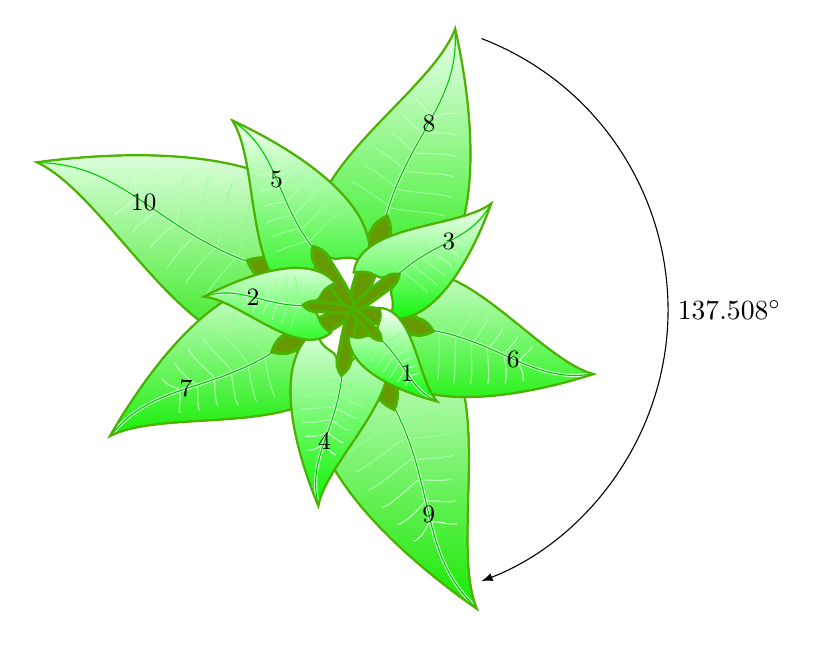
\begin{tikzpicture}
\foreach \x in {10,...,1}
{\draw[shade,bottom color=red!\x!green,top color=green!\x,x=0.3 pt,y=0.3 pt,scale={0.4+0.1*\x},rotate=222.5*\x] (0,0) .. 
controls ( -11,  1) and ( -9, 50) .. (-10,80) ..
controls ( -16, 60) and (-32, 75) .. (-50,40) .. 
controls (-110,100) and (-0,230) ..  (  0,300)  node[below] (\x) {} ..
controls (  45,230) and (110,100) .. ( 50,40) ..
controls (  32, 75) and ( 16, 60) ..  ( 10,80) ..
controls (   9, 50) and ( 11,  1) .. (  0,0) 
-- cycle ;

\draw[thin,green!45,x=0.3 pt,y=0.3 pt,scale={0.4+0.1*\x},rotate=222.5*\x] (-45,120) .. controls (-35,120) and (0,110) .. (-3,110) .. controls (0,105) and (40,120) .. (55,120);
\draw[thin,green!40,x=0.3 pt,y=0.3 pt,scale={0.4+0.1*\x},rotate=222.5*\x] (-40,140) .. controls (-30,140) and (0,130) .. (-3,130) .. controls (0,125) and (40,140) .. (55,140);
\draw[thin,green!35,x=0.3 pt,y=0.3 pt,scale={0.4+0.1*\x},rotate=222.5*\x] (-35,160) .. controls (-25,160) and (0,150) .. (0,150) .. controls (0,145) and (35,160) .. (50,160);
\draw[thin,green!30,x=0.3 pt,y=0.3 pt,scale={0.4+0.1*\x},rotate=222.5*\x] (-25,180) .. controls (-17,180) and (0,170) .. (3,170) .. controls (0,165) and (30,180) .. (45,180);
\draw[thin,green!25,x=0.3 pt,y=0.3 pt,scale={0.4+0.1*\x},rotate=222.5*\x] (-20,200) .. controls (-13,200) and (0,190) .. (6,190) .. controls (0,185) and (20,200) .. (38,200);
\draw[thin,green!20,x=0.3 pt,y=0.3 pt,scale={0.4+0.1*\x},rotate=222.5*\x] (-13,220) .. controls (-8,220) and (3,210) .. (8,210) .. controls (10,205) and (18,220) .. (30,220);
\draw[very thick,green!20,x=0.3 pt,y=0.3 pt,scale={0.4+0.1*\x},rotate=222.5*\x] (0,90) .. controls (-10,180) and (30,230) .. (1,297);
\draw[thin,black!20!green,x=0.3 pt,y=0.3 pt,scale={0.4+0.1*\x},rotate=222.5*\x] (0,90)  .. controls (-10,180) and (30,230)  .. (1,297) node[midway,black] (num\x) {\small\x};
\draw[very thick,red!30!green,fill=red!40!green,x=0.3 pt,y=0.3 pt,scale={0.4+0.1*\x},rotate=222.5*\x] 
(0,0) .. 
controls ( -11,  1) and ( -9, 50) ..
(-10,80) .. 
controls (-10,90) and (0,100) .. (0,100) ..
controls (0,100) and (10,90) .. (10,80)..
controls (   9, 50) and ( 11,  1) .. (  0,0) 
-- cycle;
\draw[thick,red!30!green,x=0.3 pt,y=0.3 pt,scale={0.4+0.1*\x},rotate=222.5*\x] (0,0) .. 
controls ( -11,  1) and ( -9, 50) .. (-10,80) ..
controls ( -16, 60) and (-32, 75) .. (-50,40) .. 
controls (-110,100) and (-0,230) ..  (  0,300) ..
controls (  45,230) and (110,100) .. ( 50,40) ..
controls (  32, 75) and ( 16, 60) ..  ( 10,80) ..
controls (   9, 50) and ( 11,  1) .. (  0,0) 
-- cycle ;
}
\draw[->,>=latex,x=0.3 pt,y=0.3 pt,black] ([xshift=6pt] 8.east) arc (69:-69:350) node[midway,right] {$137.508^\circ$};
\end{tikzpicture}
\end{document}